\chapter{Convección Mixta en Flujos Completamente Desarrollado}


La finalidad de este capítulo es que el lector/jurado comprenda la forma de abordar el problema estudiado. Así como las magnitudes y parámetros relevantes del problema. 


\newpage

\section{Casos simulados} 

Los resultados de las simulaciones realizadas en este capítulo corresponden a un flujo completamente desarrollado tanto térmica como hidrodinámicamente. Se utilizaron valores de números adimensionales tales que Re$_o$=2100, 3150, 4278, 5000, Pr=0.071, 0.71 y valores de Richardon en el rango 0.04 $\lesssim$ Ri$_b$ $\lesssim$ 106. En la Figura \ref{fig:map_flow_regime} se expone un ``mapa'' del régimen de flujo donde se gráfica el número de Reynolds\footnote{Número de Reynolds basado en el diámetro hidráulico: $Re^D_b = 8/3 \hspace*{1mm} Re_o$} versus el número de Richardson. De acuerdo al diagrama de Moody \cite{white}:

\begin{itemize}
	\item para valores de Re$^D_b$ $<$ 2000 el régimen es laminar,
	\item si 2000 $\lesssim$ Re$^D_b$ $\lesssim$ 4000 el régimen es de transición,
	\item y si Re$^D_b>$ 4000 el régimen es turbulento.
\end{itemize}
Por otra parte, el fenómeno de convección es \cite{incropera,cengelheat}:

\begin{itemize}
	\item forzado si Ri$_b<$ 0.1,
	\item mixto si 0.1 $<$ Ri$_b$ $<$10,
	\item y natural si Ri$_b$ $>$10.
\end{itemize}

\begin{figure}[H]
  \centering
    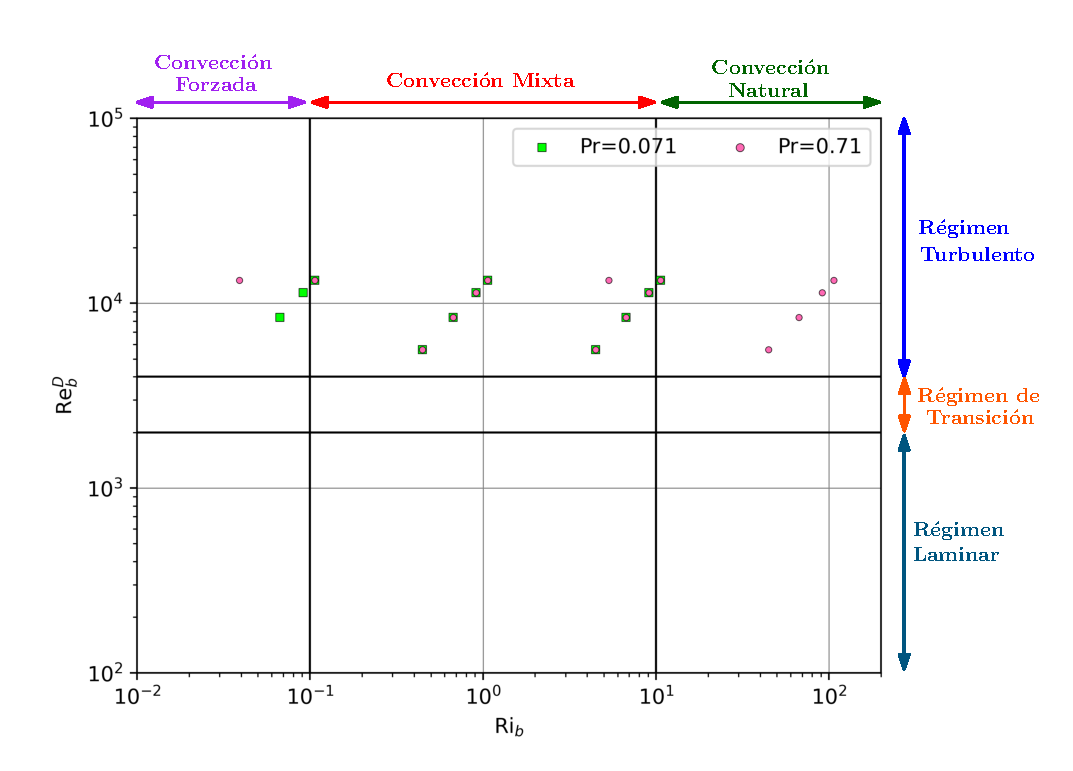
\includegraphics[width=0.7\textwidth]{figures/cap5/map.eps}
  \caption{Mapa de regímenes de los casos simulados.}
  \label{fig:map_flow_regime}
\end{figure}

La totalidad de casos se encuentra en un régimen de flujo turbulento. En su mayoría, los casos se encuentran en flujo de convección mixta, sin embargo, contamos con casos donde predomina la convección forzada, y por otro lado, donde domina la convección natural. Esto brinda un espectro más amplio para el análisis del problema.



\section{Magnitudes de Primer y Segundo Orden}

En esta sección, se pretende analizar la influencia de la fuerza boyante en las magnitudes estadísticas de primer y segundo orden. Para tal fin, se consideran, únicamente, los casos Re$_o$=5000 y Pr=0.71 . El aumento de la fuerza boyante, o el número de Ri$_b$, equivale a aumentar el flujo de calor ya que Ri$_b$ $\propto$ $q''_w$. En otras palabras, el aumento de la boyancia en este sistema físico corresponde a aumentar la energía térmica que se le entrega a través de las paredes cuando el fluido es ascendente\footnote{También es equivalente a quitarle energía térmica (enfriar las paredes) cuando la dirección del flujo es descendente.}.


\subsection{Perfiles de velocidad y de temperatura} \label{sec:velo_temp}

En la Figura \ref{fig:ux-Re5000-Pr071} se presenta los perfiles de velocidad (\textit{streamwise}) para los diferentes números de Richardson. En él, es posible distinguir claramente los tres régimenes de convección. Cerca de las paredes, la temperatura del fluido es mayor y por tanto, es más liviano que el fluido que se encuentra en el centro del canal. En este sentido, existe un gradiente de densidad, que bajo la acción de la gravedad, se traduce en un aumento de la velocidad (debido a la fuerza boyante) que eleva el fluido más caliente cerca de la pared. A su vez, esto produce un arrastre de fluido desde el seno del canal hacia las paredes promoviendo la mezcla del mismo.

\begin{figure}[H]
  \centering
  \subfloat[]{
    \includegraphics[width=0.49\textwidth]{figures/cap5/Re5000-Pr071/phi_mean_profile.png}
    	\label{fig:phi-Re5000-Pr071}}
  \subfloat[]{
    \includegraphics[width=0.49\textwidth]{figures/cap5/Re5000-Pr071/ux_mean_profile.png}
    	\label{fig:ux-Re5000-Pr071}}
  \caption{}
\end{figure}

Esta mezcla, ayuda a redistribuir la energía térmica sumistrada, y por lo tanto, es la responsable de que la temperatura a lo largo del canal sea más uniforme, dando lugar a esa forma``achatada'' en el centro, en comparación al caso forzado, tal como se observa en los perfiles de temperatura expuestos en la Figura \ref{fig:phi-Re5000-Pr071}. Aquí, los casos se pueden dividir, a priori, en dos grupos: el primer grupo que corresponde a valores de Rib$_b$ entre 0.04 y 1.06, y el segundo grupo está compuesto por valores de 5.33 a 106.5 . En el primer grupo, se produce un aumento de temperatura en el seno del fluido que reduce la transferencia de calor (como se verá en la sección \ref{sec:nu}). En el segundo grupo, se produce un descenso de la temperatura en el seno del fluido mejorando la transferencia de calor. En ese sentido, el sistema es más eficiente para ``evacuar'' el calor suministrado a medida que Ri$_b$ (o $q''_w$) es más alto. Esto genera una disminución en la temperatura de las paredes y desde el punto de vista ingenieríl, puede ser útil para sistemas de refrigeración. 

%Estas últimas afirmaciones, que a priori resultan no evidentes, pueden entenderse a partir de la Figura \ref{fig:uphi-Re5000-Pr071}. En ella, se muestra el perfil de la magnitud $\langle u_x^* \theta^* \rangle$. El número de Nusselt es inversamente proporcional a $\langle \theta^*_b \rangle = \frac{\int_A \langle u_x* \theta^* \rangle dA}{U_b} $ donde la velocidad \textit{bulk} $U_b$ es constante, ya que se mantiene fijo el caudal. Se puede observar, que el aumento de la temperatura en en el seno del canal conlleva a un aumento del $\langle u_x^* \theta^* \rangle$, por consiguiente de $$\langle \theta^*_b \rangle$ y por lo tanto una disminución de Nu. 

\begin{figure}[H]
  \centering
    \includegraphics[width=0.6\textwidth]{figures/cap5/Re5000-Pr071/uphi_profile.png}
 	 \caption{}
  \label{fig:uphi-Re5000-Pr071}
\end{figure}

Estas afirmaciones, que no son evidentes a primera vista, se comprenden a partir de la Figura \ref{fig:uphi-Re5000-Pr071}, donde se muestra el perfil de $\langle u_x^{*} \theta^{*} \rangle$. El número de Nusselt es inversamente proporcional a
$$\langle \theta^*_b \rangle = \frac{ \frac{1}{A} \int_A \langle u_x^* \theta^* \rangle dA}{U_b} $$
y la velocidad \textit{bulk} $U_b$ es constante porque el caudal se mantiene fijo. Así, un incremento de la temperatura en el seno del canal aumenta $\langle u_x^{*} \theta^{*} \rangle$, y, en consecuencia, eleva $\langle \theta_b^{*} \rangle$, lo que provoca una disminución de Nu.

\subsection{Valores RMS de temperatura, velocidad y flujo turbulento de calor} 

Las Figuras \ref{fig:rms-phi-log-Re5000-Pr071} y \ref{fig:rms-ux-Re5000-Pr071} muestran, respectivamente, los perfiles de las fluctuaciones de temperatura y de velocidad en la dirección \textit{streamwise}. A primera vista, al aumentar el número de Richardson, las fluctuaciones de temperatura disminuyen mientras que las de velocidad aumentan, lo cual se aprecia sobre todo en los casos de Ri$_b$ más elevados. No obstante, para Ri$_b = 0{.}04$, $0{.}11$ y $1{.}06$ la evolución difiere: primero se observa una reducción (incremento) de las fluctuaciones de velocidad (temperatura) seguida de una ligera recuperación (caída) antes de alinearse con la tendencia general del resto de los casos. Este comportamiento particular también fue reportado en otro trabajo \cite{you2003direct}.

El incremento de $(u_x^*)_{rms}$ con la fuerza boyante sugiere que el flujo adquiere un carácter más caótico, y por ende, más turbulento, lo que potencia la mezcla y genera un ``recambio'' continuo de fluido que atenúa las fluctuaciones de temperatura.

\begin{figure}[H]
  \centering
  \subfloat[]{
    \includegraphics[width=0.49\textwidth]{figures/cap5/Re5000-Pr071/phi_rms_profile.png}
    	\label{fig:rms-phi-log-Re5000-Pr071}}
  \subfloat[]{
    \includegraphics[width=0.49\textwidth]{figures/cap5/Re5000-Pr071/ux_rms_profile.png}
    	\label{fig:rms-ux-Re5000-Pr071}}
  \caption{}
\end{figure}

La Figura \ref{fig:uphif-Re5000-Pr071} muestra el perfil de la correlación $\langle u_x^{*'} \theta^{*'} \rangle$. Dado que el flujo de calor convectivo obedece, en primer orden, a $q'' \simeq \rho \hspace{0.5mm} c_P \hspace{0.5mm} U \hspace{0.5mm} \Delta T$, esta correlación puede interpretarse como proporcional al flujo de calor turbulento en la dirección $x$, es decir, al calor transportado por las estructuras turbulentas del flujo \cite{kundu, pope2001turbulent}. Para valores de Ri$_b$ próximos a cero (es decir, la convección forzada predomina), dichas estructuras trasportan el calor sobre todo en las proximidades de las paredes. Sin embargo, al aumentar la fuerza boyante, el signo de $\langle u_x^{*'} \theta^{*'} \rangle$ se invierte en la región central del canal: el flujo de calor turbulento se orienta contracorriente, de modo que regiones más frías de fluido son arrastradas aguas abajo. Este mecanismo disminuye la eficiencia global de la transferencia de calor.


\begin{figure}[H]
  \centering
   \includegraphics[width=0.6\textwidth]{figures/cap5/Re5000-Pr071/uphif_profile.png}
   	\label{fig:uphif-Re5000-Pr071}
  \caption{}
\end{figure}


\section{Comparación entre casos de distinto Prandtl}

%En esta sección se compara los casos con Re$_o$=5000 y Pr=0.071,0.71. La Figura \ref{fig:plus-ux-Re5000-Prs} presenta lo perfiles de velocidad media en términos de \textit{wall units}. En la subcapa viscosa ($y^+ < 5$), es posible aproximar la velocidad como $\langle u_x^+ \rangle \simeq y^+ + \mathcal{O}((y^+)^2)$ \cite{pope2001turbulent}, cuya dicha aproximación está representada con la linea negra del gráfico. En esta región, el tensor de esfuerzo de Reynolds es despreciable comparado con el tensor de esfuerzo viscoso. En efecto, se puede apreciar que independientemente de la sustancia y de fuerza boyante, todos los casos muestran ser consistentes con dicha aproximación.

En esta sección se comparan los casos con $Re\_o = 5000$ y Pr = 0.071 y 0.71. La Figura \ref{fig:plus-ux-Re5000-Prs} muestra los perfiles de velocidad media expresados en unidades de pared (\textit{wall units}). En la subcapa viscosa ($y^+ < 5$) la velocidad puede aproximarse por
$$\langle u_x^+ \rangle \;\simeq\; y^+ + \mathcal{O} \left[(y^+)^{2} \right],$$
según Pope \cite{pope2001turbulent}. Esta ley se indica en la figura con la línea negra de referencia. En dicha región las tensiones de Reynolds son despreciables frente a las tensiones viscosas, de modo que el perfil depende casi exclusivamente de la distancia normalizada a la pared. Como puede verse, todos los casos, independientemente del número de Prandtl y de la fuerza de flotación, siguen de cerca esta aproximación lineal, lo que confirma la validez de la ley en la subcapa viscosa.

\begin{figure}[H]
  \centering
    \subfloat[]{
    \includegraphics[width=0.5\textwidth]{figures/cap5/ux_mean_plus_log_profile.png}
  	  	\label{fig:plus-ux-Re5000-Prs}}
 	 \subfloat[]{
    \includegraphics[width=0.5\textwidth]{figures/cap5/phi_mean_plus_log_profile.png}
    	\label{fig:plus-phi-log-Re5000-Prs}}
  \caption{}
  \label{fig:Re5000-Pr071}
\end{figure}

%Por otra parte, en la Figura \ref{fig:plus-phi-Re5000-Prs} se presentan lo perfiles de temperatura media. Es posible aproximar la variación de la temperatura media cerca de la pared como proporcional a $y^+$ \cite{kawamura1998dns}:
%
%\begin{equation*}
%\langle \theta^* \rangle \simeq \text{Pr}\hspace{0.5mm} y^+
%\end{equation*}
% 
%Esta aproximación está representada en el gŕafico con lineas negras. Podemos ver que los casos con distinto Pr dicha aprox se corresponde con los datos de la simulación. Se aprecia que para el Pr más bajo la ley tiene un buen hasta $y^+ \sim 13$ mientras que para el más alto es menor, $y^+ \sim 7$. Esto está relacionado al hecho de que el fenómeno de conducción cerca la pared es más relevante que la convección para fluidos con difusividad térmica o Pr más bajos \cite{abregu2023dns}.



Por otra parte, la Figura \ref{fig:plus-phi-Re5000-Prs} muestra los perfiles de temperatura media en unidades de pared. Cerca de la pared, la variación de la temperatura puede aproximarse por la relación lineal \cite{kawamura1998dns}
\begin{equation*}
\langle \theta^* \rangle \simeq \text{Pr}\hspace{0.5mm} y^+ ,
\end{equation*}
representada en la figura con líneas negras. Los resultados confirman esta ley para ambos números de Prandtl, aunque con distintos alcances: para el caso de Pr=0.071 la validez se extiende hasta $y^{+}\approx 13$, mientras que para Pr=0.71 se reduce a $y^{+}\approx 7$. La diferencia se debe a que, en fluidos con menor difusividad térmica (Prandtl más bajo), el transporte de calor por conducción domina durante una mayor distancia normalizada desde la pared, retrasando la aparición del régimen convectivo predominante \cite{abregu2023dns}.






%\section{UHF vs UWT}
%
%En la sección [REF-VALIDACIONES] se utilizaron las simulaciones obtenidas por Guo y Prasser \cite{guo2022direct} para validar la herramienta numérica utilizada. El sistema estudiado por dichos autores corresponde a una configuración física distinta que al sistema estudiado en este trabajo, sin embargo, resulta útil comparar los perfiles de velocidad y temperatura, para entender en mayor profundidad el fenómeno de convección. En esta sección se pretende cotejar las dos configuraciones físicas establecidas: UHF\footnote{\textit{Uniform Heat Flux}} y UWT\footnote{\textit{Uniform Wall Temperature}}. El primero corresponde a los parámetros Re$_o$=3150, Pr=0.071 y Ri$_b$=0.67, y el segundo, a Re$_o$=3500, Pr=0.025 y Ri$_b$=0.5. Si bien los parámetros involucrados no son idénticos, están en el mismo orden de magnitud, para fines cualitativos, esto es más que adecuado para análizar la física detrás de ellos. Las Figuras \ref{fig:guocomp_ux} y \ref{fig:guocomp_phi} exponen los perfiles de velocidad en la dirección de la corriente y la temperatura de ambas configuraciones, respectivamente. En ambos casos se normaliza los perfiles con el máximo de la propia curva.  
%
%\begin{figure}[H]
%  \centering
%  \subfloat[]{
%    \includegraphics[width=0.49\textwidth]{figures/cap5/phi_mean_profile.png}
%    	\label{fig:guocomp_ux}}
%  \subfloat[]{
%    \includegraphics[width=0.49\textwidth]{figures/cap5/ux_mean_profile.png}
%    	\label{fig:guocomp_phi}}
%  \caption{Comparación entre los dos problemas.}
%  \label{fig:ux-guocomp}
%\end{figure}
%
%
%Una característica inmediata que se observa recae en la asimetría del los perfiles del caso UWT en comparación con UHF, lo que resulta claro debido a la asimetría del primero con respecto al segundo caso. 
%
%
%\textcolor{magenta}{seguir explicando la fisica de ambos casos.}



%\newpage
%\section{Número de Nusselt} \label{sec:nu}
%
%Desde una perspectiva ingenieríl, un parámetro importante que da información sobre la eficiencia de la transferencia de calor es el número de Nusselt (Nu), el cuál se define en la ecuación \ref{eq:nu}, donde $\overline{\theta_b}$ es la temperatura en \textit{bulk}.
%
%Un parámetro importante desde una perspectiva ingenieríl es el número de Nusselt (Nu), el cuál se define en la ecuación \ref{eq:nu}, donde $\overline{\theta_b}$ es la temperatura en \textit{bulk} (ecuación \ref{eq:tita_bulk}).
%
%\begin{equation}
%\text{Nu} = \frac{h L}{k} = \frac{2d \hspace*{1mm} q''_w}{k \hspace*{1mm} \overline{\theta^*_b}} = \frac{4}{3} \frac{Re_o Pr}{\overline{\theta^*_b}}	
%\label{eq:nu}
%\end{equation}
%
%\begin{equation*}
%\overline{\theta_b} = \frac{\frac{1}{A} \int \langle u_x \theta \rangle }{U_b} = \frac{\int^d_0 \langle u_x \theta \rangle \hspace*{0.5mm} dy }{\int^d_0 \langle u_x \rangle \hspace*{0.5mm} dy}
%\label{eq:tita_bulk}
%\end{equation*}
%
%En la Figura \ref{fig:nu_vs_bo} se presentan todos los valores de Nu obtenidos, graficados en función del número de boyancia Bo, definido en la ecuación \ref{eq:jackson_bo}, el cuál da una idea del \textit{ratio} entre las intensidad de las fuerzas boyantes y el la fuerza impulsora de la convección forzada. Los valores se contrastan con la correlación de Jackson et al. \cite{jackson1989studies}, expresada en la ecuación \ref{eq:jackson_corr}. Los valores Nu están normalizados con el Nu de convección forzada puro Nu$_{fc}$ el cuál es obtenido a partir de la correlación de Dittus-Boelter \cite{incropera}. Además, se añaden otros valores de Nu obtenidos mediante simulaciones DNS \cite{you2003direct} a modo de comparativa y se puede observar que los mismos se alinean con la tendencia de la correlación al igual que nuestro caso. 
%
%En la Figura \ref{fig:parity} se muestra un gráfico de paridad entre los números de Nusselt obtenidos por DNS, $Nu_{\text{DNS}}/Nu_{DB}$ (eje $x$), y los calculados con la correlación de Jackson, $Nu_{\text{corr}}/Nu_{DB}$ (eje $y$). La línea negra representa el acuerdo perfecto ($y=x$), mientras que las líneas azules punteadas señalan la banda de $\pm2\sigma$ alrededor de esa bisectriz. Puede verse que prácticamente todos los puntos experimentales se agrupan muy cerca de la bisectriz y permanecen dentro de la banda de $\pm2\sigma$, evidenciando que la correlación de Jackson reproduce con buena precisión los valores simulados a lo largo de todo el rango de $Nu_{\text{DNS}}/Nu_{DB}$ considerado.
%
%
%Pueden distinguir 3 regiones principales
%\begin{itemize}
% \item[$\bullet$] para Bo $\lesssim$ $10^{-6}$ el valor Nu es practicamente igual a Nu$_{fc}$, es decir, domina la convección forzada,
% \item[$\bullet$] en el rango $10^{-6}$ $\lesssim$ Bo $\lesssim$ $3 \times 10^{-5}$ se observa una caida y una recuperación del número de Nusselt, revelando la existencia de una región donde la transferencia de calor empeora por debajo del caso únicamente forzada y que luego retoma su condición original,
% \item[$\bullet$] por último, para Bo $\gtrsim$ $3 \times 10^{-5}$ la transferencia de calor aumenta notoriamente, impulsado por las corrientes de convección natural que en esta región tiene mayor preponderancia.
%\end{itemize}
%
%%\vspace*{-1.5cm}
%
%\begin{equation}
%\text{Bo}= \frac{Gr*}{{\text{Re}_D}^{3.425} \hspace*{1mm} \text{Pr}^{0.8} }
%\label{eq:jackson_bo}
%\end{equation}
%
%\begin{equation}
%\frac{\text{Nu}}{\text{Nu}_{fc}}= \left\vert  1 - 8 \times 10^4 \hspace*{0.5mm} \text{Bo} \hspace*{0.5mm} \left( \frac{\text{Nu}}{\text{Nu}_{fc}} \right)^{-2}  \right\vert^{0.46}
%\label{eq:jackson_corr} 
%\end{equation}
%
%
%\begin{figure}[H]
%  \centering
%  \subfloat[]{
%    \includegraphics[width=0.49\textwidth]{figures/cap5/nusselt_corr/Nu_vs_Bo_Jackson.png}
%    	\label{fig:nu_vs_bo}}
%  \subfloat[]{
%    \includegraphics[width=0.49\textwidth]{figures/cap5/nusselt_corr/jackson_parity.png}
%    	\label{fig:parity}}
%    
%  \caption{Aquí $Bo = Gr / (Re^{3,425} Pr^{0,8})$}
%  \label{fig:nusselt}
%\end{figure}
%
%La caída del número de Nu con el aumento de la fuerza boyante puede interpretarse en términos del perfil de velocidad en la dirección de la corriente. En la sección \ref{sec:velo_temp} se comentó que cuando la convección natural y la convección forzada actúan en la misma dirección el fluido es acelerado en las zonas cercanas a las paredes y, en virtud de la conservación de masa, el flujo se desacelera en la región central. En virtud de esta premisa es posible acercarse a un entendimiento cualitativo. De acuerdo al modelo de Prandtl \cite{Prandtl1942}, la transferencia de calor ocurre mediante 2 mecanísmo principales: transferencia por conducción en la subcapa viscosa y por el flujo de calor turbulento en la dirección normal a la pared, esto es, $q''_y \aprox \rho \hspace{0.5mm} c_P \hspace{0.5mm} \langle u^{*'}_y \theta^{*'} \rangle$. De acuerdo a Aicher y Martin \cite{aicher1997}, en la zona cercana al borde de la capa viscosa, el flujo $q''_y$ es proporcional a la producción de turbulencia el cuál es la suma de la \textit{Shear-Production} y \textit{Buoyancy-Production}, cantidades (o \textit{budgets}) provenientes del balance de la cinética turbulenta $k$ (Apéndice \ref{apen:budgets}). En este sentido, la producción de turbulencia dependerá de la diferencia de velocidades entre el centro del canal y la zona próxima a la pared.
%
%Así, dado que la boyancia produce un aumento de la velocidad cerca de las paredes, es posible apreciar una rango de Ri$b$ ($10^{-6}$ $\lesssim$ Bo $\lesssim$ $3 \times 10^{-5}$ de la Figura \ref{fig:nu_vs_bo}) para los cuales ésta diferencia es, o bien cero, o bien muy pequeña. A medida que la fuerza boyante sigue incrementando, dicha diferencia de velocidades (o gradiente) crece, y en consecuencia, aumenta la producción de turbulencia, el flujo de calor turbulento normal y transferencia de calor que se refeja en un aumento del Nu.  
%
%
%
%


%\begin{figure}[H]
%  \centering
%   \includegraphics[width=0.6\textwidth]{figures/cap5/Re5000-Pr071/uphif_profile.png}
%   	\label{fig:uphif-Re5000-Pr071}
%  \caption{\textcolor{red}{Acá va el flujo de calor turbulento normal a la pared ... solo que todavía no pude hacerlo porque el cluster está inactivo ...}}
%\end{figure}


\newpage
\section{Número de Nusselt} \label{sec:nu}

Desde una perspectiva ingenieril, el número de Nusselt (Nu) es un indicador clave de la eficiencia de la transferencia de calor. Su definición se presenta en la ecuación \ref{eq:nu}, donde $\langle \theta_b \rangle$ es la temperatura \textit{bulk} (ecuación \ref{eq:tita_bulk}).

\begin{equation}
\text{Nu} = \frac{h L}{k} = \frac{2d \hspace*{1mm} q''_w}{k \hspace*{1mm} \langle \theta^*_b \rangle} = \frac{4}{3} \frac{Re_o Pr}{\langle \theta^*_b \rangle}	
\label{eq:nu}
\end{equation}

\begin{equation}
\langle \theta_b \rangle = \frac{\frac{1}{A} \int \langle u_x \theta \rangle }{U_b} = \frac{\int_0^d \langle u_x \theta \rangle \, dy}{\int_0^d \langle u_x \rangle \, dy}
\label{eq:tita_bulk}
\end{equation}

La Figura \ref{fig:nu_vs_bo} muestra los valores de Nu obtenidos en función del número de boyancia Bo (ecuación \ref{eq:jackson_bo}), que cuantifica la relación entre las fuerzas boyantes y la fuerza impulsora de la convección forzada. Estos resultados se comparan con la correlación de Jackson et al. \cite{jackson1989studies} (ecuación \ref{eq:jackson_corr}). Todos los valores de Nu se normalizan con el valor correspondiente a convección forzada pura, Nu$_{fc}$, evaluado mediante la correlación de Dittus-Boelter \cite{incropera}. También se añaden datos provenientes de simulaciones DNS \cite{you2003direct}, que se alinean con la misma tendencia.

En la Figura \ref{fig:parity} se presenta un gráfico de paridad entre $Nu_{\text{DNS}}/Nu_{DB}$ (eje $x$) y $Nu_{\text{corr}}/Nu_{DB}$ (eje $y$). La línea negra indica el acuerdo perfecto ($y=x$) y las líneas azules punteadas delimitan la banda de $\pm2\sigma$ (con $\sigma$=0.158). La concentración de puntos dentro de esta banda confirma que la correlación de Jackson reproduce con buena precisión los valores simulados.

A partir de la Figura \ref{fig:nu_vs_bo} se distinguen tres regiones:

\begin{itemize}
  \item[$\bullet$] Bo $\lesssim 10^{-6}$: Nu se mantiene prácticamente igual a Nu$_{fc}$; domina la convección forzada.
  \item[$\bullet$] $10^{-6} \lesssim$ Bo $\lesssim 3 \times 10^{-5}$: Nu desciende y luego se recupera, indicando una zona donde la transferencia de calor empeora temporalmente respecto al caso puramente forzado.
  \item[$\bullet$] Bo $\gtrsim 3 \times 10^{-5}$: Nu crece de forma marcada, impulsado por la mayor relevancia de la convección natural.
\end{itemize}

\begin{equation}
\text{Bo}= \frac{Gr*}{\text{Re}_D^{3.425} \hspace*{1mm} \text{Pr}^{0.8}}
\label{eq:jackson_bo}
\end{equation}

\begin{equation}
\frac{\text{Nu}}{\text{Nu}_{fc}} =
\left\vert 1 - 8 \times 10^4 \hspace*{0.5mm} \text{Bo}
\left( \frac{\text{Nu}}{\text{Nu}_{fc}} \right)^{-2} \right\vert^{0.46}
\label{eq:jackson_corr}
\end{equation}

\begin{figure}[H]
  \centering
  \subfloat[]{
    \includegraphics[width=0.49\textwidth]{figures/cap5/nusselt_corr/Nu_vs_Bo_Jackson.png}
    \label{fig:nu_vs_bo}}
  \subfloat[]{
    \includegraphics[width=0.49\textwidth]{figures/cap5/nusselt_corr/jackson_parity.png}
    \label{fig:parity}}
  \caption{Número de boyancia: $Bo = Gr / (Re^{3.425} Pr^{0.8})$.}
  \label{fig:nusselt}
\end{figure}



La disminución de Nu al aumentar la fuerza boyante puede entenderse a partir del perfil de velocidad en la dirección del flujo. Como se menciona en la sección \ref{sec:velo_temp}, cuando la convección natural y forzada actúan en la misma dirección, el fluido se acelera junto a las paredes y, por conservación de masa, se desacelera en la región central. En virtud de esta premisa, es posible acercarse a un entendimiento cualitativo. De acuerdo al modelo de Prandtl \cite{Prandtl1942}, la transferencia de calor se divide en dos mecanismos principales: (i) conducción en la subcapa viscosa y (ii) flujo de calor turbulento normal a la pared, $q''_y \approx \rho \, c_P \, \langle u^{*'}_y \theta^{*'} \rangle$. De acuerdo Aicher y Martin \cite{aicher1997}, justo en el borde de la subcapa viscosa, $q''_y$ es proporcional a la producción de turbulencia, definida como la suma de \textit{Shear-Production} y \textit{Buoyancy-Production} (véase Apéndice \ref{apen:budgets}). Esta producción depende de la diferencia de velocidades entre el centro del canal y la zona próxima a la pared\footnote{Esto último puede ser entendido como un gradiente de velocidad}.  

Así, es posible apreciar una rango de Ri$b$, correspondiente al intervalo $10^{-6}$ $\lesssim$ Bo $\lesssim$ $3 \times 10^{-5}$ en la Figura \ref{fig:nu_vs_bo}, para los cuales la aceleración inducida por la boyancia produce que esta diferencia, o bien sea cero, o bien sea muy pequeña. Como consecuencia, disminuyen la producción turbulenta, el flujo de calor turbulento y, por lo tanto, Nu. Cuando la fuerza boyante continúa creciendo más allá de este intervalo, el gradiente de velocidad vuelve a incrementarse, la producción de turbulencia se intensifica y tanto $q''_y$ como Nu aumentan nuevamente.

\newpage
\section{Factor de Fricción de Darcy}

\begin{figure}[H]
  \centering
  \subfloat[]{
    \includegraphics[width=0.7\textwidth]{figures/cap5/nusselt_corr/darcy_vs_Bo.png}}
  \caption{Factor de Darcy $ f$. Aquí $Bo = Gr / (Re^{3,425} Pr^{0,8})$}
  \label{fig:darcy_vs_bo}
\end{figure}

